% !TeX program = xelatex
% Khoa hoc may nang cao 2026: review-guided, report-aligned edition.
\documentclass[10pt,aspectratio=43]{beamer}
\usepackage{fontspec}
\setsansfont{lmsans10-regular.otf}[BoldFont=lmsans10-bold.otf,ItalicFont=lmsans10-oblique.otf,BoldItalicFont=lmsans10-boldoblique.otf]
\setmainfont{lmsans10-regular.otf}[BoldFont=lmsans10-bold.otf,ItalicFont=lmsans10-oblique.otf,BoldItalicFont=lmsans10-boldoblique.otf]
\usepackage[vietnamese]{babel}
\usepackage{amsmath,amssymb,mathtools,booktabs,array,tabularx,multirow}
\usepackage[table]{xcolor}
\usepackage{tikz}
\usetikzlibrary{arrows.meta,positioning,shapes.geometric,calc,fit}
\usepackage{graphicx}
% Beamer theme -- no grey "Nguon" lines (at the user's request).
\usetheme{Boadilla}
\useoutertheme{miniframes}
\useinnertheme{circles}
\definecolor{PrimaryBlue}{RGB}{24,48,111}
\definecolor{SecondaryBlue}{RGB}{25,100,157}
\definecolor{PaleBlue}{RGB}{233,244,251}
\definecolor{LightGray}{RGB}{245,248,250}
\definecolor{AccentOrange}{RGB}{190,91,25}
\definecolor{AccentGreen}{RGB}{14,113,103}
\setbeamercolor{normal text}{fg=black,bg=white}
\setbeamercolor{structure}{fg=PrimaryBlue}
\setbeamercolor{title}{fg=PrimaryBlue}
\setbeamercolor{frametitle}{fg=PrimaryBlue,bg=white}
\setbeamercolor{block title}{fg=white,bg=PrimaryBlue}
\setbeamercolor{block body}{fg=black,bg=PaleBlue}
\setbeamercolor{alerted text}{fg=AccentOrange}
\setbeamercolor{palette primary}{bg=PrimaryBlue,fg=white}
\setbeamercolor{palette secondary}{bg=SecondaryBlue,fg=white}
\setbeamercolor{palette tertiary}{bg=PrimaryBlue,fg=white}
\setbeamercolor{palette quaternary}{bg=PrimaryBlue,fg=white}
\setbeamercolor{section in head/foot}{bg=PrimaryBlue,fg=white}
\setbeamercolor{subsection in head/foot}{bg=SecondaryBlue,fg=white}
\setbeamercolor{author in head/foot}{bg=PrimaryBlue,fg=white}
\setbeamercolor{title in head/foot}{bg=SecondaryBlue,fg=white}
\setbeamercolor{date in head/foot}{bg=PrimaryBlue,fg=white}
\setbeamerfont{frametitle}{size=\large,series=\bfseries}
\setbeamerfont{block title}{series=\bfseries}
\setbeamertemplate{navigation symbols}{}
\setbeamertemplate{footline}{%
  \leavevmode\hbox{%
  \begin{beamercolorbox}[wd=.20\paperwidth,ht=2.4ex,dp=1.1ex,center]{author in head/foot}Học máy nâng cao\end{beamercolorbox}%
  \begin{beamercolorbox}[wd=.65\paperwidth,ht=2.4ex,dp=1.1ex,center]{title in head/foot}Khuyến nghị sản phẩm điện tử -- GRNR \& DFHF\end{beamercolorbox}%
  \begin{beamercolorbox}[wd=.15\paperwidth,ht=2.4ex,dp=1.1ex,right]{date in head/foot}\insertframenumber/\inserttotalframenumber\hspace*{1.5ex}\end{beamercolorbox}}%
  \vskip0pt}
\setbeamersize{text margin left=0.6cm,text margin right=0.6cm}
\setlength{\parskip}{0.6pt}
\newcommand{\takeaway}[1]{%
\par\vspace{0.12cm}%
\begin{beamercolorbox}[rounded=true,sep=4pt]{block body}%
\footnotesize\textbf{Ý chính:} #1%
\end{beamercolorbox}}
\newcommand{\metric}[2]{%
\begin{block}{\centering\Large\bfseries #1}\centering\footnotesize #2\end{block}}
\newcommand{\shortnote}[1]{\vspace{0.1cm}\centerline{\footnotesize\color{PrimaryBlue}\textbf{#1}}}

\definecolor{CoverBlue}{RGB}{25,48,106}
\title[Khuyến nghị sản phẩm điện tử]{Hệ thống khuyến nghị sản phẩm điện tử bằng hồi quy lân cận và khuếch tán trên đồ thị}
\author[Nhóm thực hiện]{Đặng Anh Tuyền \and Phạm Văn Sự \and Nguyễn Chí Tài}
\institute[Phenikaa]{Đại học Phenikaa -- Trường Công nghệ Thông tin\\[3pt]GVHD: PGS.TS. Phạm Tiến Lâm}
\date{Hà Nội, 2026}
\begin{document}
\begin{frame}[plain]
\centering
\vspace*{0.28cm}
{\small\bfseries\color{PrimaryBlue}BỘ GIÁO DỤC VÀ ĐÀO TẠO \quad | \quad ĐẠI HỌC PHENIKAA\par}
\vspace{0.30cm}
{\footnotesize TRƯỜNG CÔNG NGHỆ THÔNG TIN\par}
\vspace{0.56cm}
\begin{tikzpicture}
\node[rounded corners=7pt,fill=CoverBlue,text=white,text width=10.55cm,
      minimum height=3.05cm,align=center,inner sep=14pt] (cover)
{\fontsize{20.3}{26}\selectfont\bfseries HỆ THỐNG KHUYẾN NGHỊ\\ SẢN PHẨM ĐIỆN TỬ\\[5pt]
 \fontsize{15.1}{20}\selectfont BẰNG HỒI QUY LÂN CẬN VÀ\\ KHUẾCH TÁN TRÊN ĐỒ THỊ};
\end{tikzpicture}
\vspace{0.25cm}
{\small Học phần: Học máy nâng cao 1-1-26 (N01)\par}
\vspace{0.3cm}
{\small Đặng Anh Tuyền \quad \quad Phạm Văn Sự \quad \quad Nguyễn Chí Tài\par}
\vspace{0.18cm}
{\small GVHD: \textbf{PGS.TS. Phạm Tiến Lâm}\par}
\vspace{0.17cm}
{\footnotesize Hà Nội, 2026\par}
\end{frame}

\begin{frame}{Nội dung trình bày}
\tableofcontents[hideallsubsections]
\end{frame}
\section{Bài toán}

\begin{frame}{Vấn đề: dữ liệu tương tác cực thưa}

\begin{columns}[T,onlytextwidth]

\begin{column}{0.30\textwidth}
    \metric{124.895}{Người dùng}
\end{column}
\hfill
\begin{column}{0.30\textwidth}
    \metric{44.843}{Sản phẩm}
\end{column}
\hfill
\begin{column}{0.30\textwidth}
    \metric{0,0192\%}{Mật độ tương tác}
\end{column}

\end{columns}
\vspace{0.28cm}
\begin{itemize}\setlength\itemsep{10pt}
\item \textbf{Lịch sử ngắn:} trung vị chỉ 6 tương tác/người dùng.
\item \textbf{Lịch sử thay đổi:} ưu tiên tính gợi ý cho lịch sử mới mà không học lại vector người dùng.
\item \textbf{MostPop là đối chứng mạnh:} phải kiểm chứng lợi ích của cá nhân hóa.
\end{itemize}
\takeaway{Đặt câu hỏi không chỉ ``mô hình nào tốt nhất'', mà còn ``khi thiếu dữ liệu, mô hình có hơn cách gợi ý phổ biến không?''}
\end{frame}

\begin{frame}{Từ lịch sử tương tác đến danh sách Top-20}
\centering
\begin{tikzpicture}[
 node distance=0.6cm,
 pbox/.style={draw=PrimaryBlue,fill=PaleBlue,rounded corners=5pt,
 text width=3.0cm,minimum height=1.5cm,align=center,font=\small,inner sep=6pt},
 edge/.style={-Latex,draw=PrimaryBlue,line width=1.5pt}]
\node[pbox] (hist) {\textbf{Lịch sử $H_u$}\\ Tai nghe, chuột, bàn phím};
\node[pbox,right=of hist] (rank) {\textbf{Điểm $s(u,i)$}\\ Xếp hạng sản phẩm ứng viên};
\node[pbox,right=of rank] (res) {\textbf{Top-20}\\ Chọn 20 sản phẩm chưa tương tác};
\draw[edge] (hist) -- (rank);
\draw[edge] (rank) -- (res);
\end{tikzpicture}
\vspace{0.30cm}
\begin{block}{Phản hồi ngầm}
\centering\small $X_{ui}=1$: đã đánh giá tích cực (\,$\ge4$ sao\,) \\
$X_{ui}=0$: \textbf{chưa quan sát}, không có nghĩa ``không thích''.
\end{block}
\vspace{0.15cm}
\begin{columns}[T,totalwidth=\textwidth]
\column{0.48\textwidth}
\begin{block}{GRNR - nhóm giải trực tiếp}\small EASE đầy đủ, EASE top-128, GF-CF.\end{block}
\column{0.48\textwidth}
\begin{block}{DFHF - cần huấn luyện}\small LightGCN, XSimGCL, DirectAU.\end{block}
\end{columns}
\shortnote{Hai nhóm được đánh giá riêng, không xếp hạng GRNR và DFHF với nhau.}
\end{frame}

\section{Phương pháp}

\begin{frame}{GRNR: Quy trình 5 bước (rút gọn)}
\centering
{\footnotesize\bfseries\color{PrimaryBlue}Khớp mô hình: từ ma trận tương tác đến trọng số sản phẩm - sản phẩm}\par
\vspace{0.32cm}
\begin{tikzpicture}[
 sbox/.style={draw=PrimaryBlue,fill=PaleBlue,rounded corners=4pt,
 minimum height=1.60cm,text width=1.65cm,align=center,font=\footnotesize,
 inner sep=3.7pt},
 sedge/.style={-Latex,draw=PrimaryBlue,line width=1.25pt}]
\node[sbox] (a) at (0,0) {\bfseries Phản hồi ngầm\\[4pt]$X$};
\node[sbox] (b) at (2.30,0) {\bfseries Chọn nguồn\\[4pt]Tối đa 128 láng giềng};
\node[sbox] (c) at (4.60,0) {\bfseries Lập đồ thị\\[4pt]Laplacian $L$};
\node[sbox] (d) at (6.90,0) {\bfseries Hồi quy\\[4pt]Trọng số $\omega_+$, chặn $b_i$};
\node[sbox] (e) at (9.20,0) {\bfseries Tham số\\[4pt]$\beta_{ij}$ và $b_i$};
\foreach \l/\r in {a/b,b/c,c/d,d/e} {\draw[sedge] (\l.east) -- (\r.west);}
\end{tikzpicture}
\vspace{0.75cm}
\begin{tikzpicture}[
 iobox/.style={draw=AccentGreen,fill=AccentGreen!8,rounded corners=4pt,
 minimum height=1.1cm,text width=3.15cm,align=center,font=\small,inner sep=5pt},
 arr/.style={-Latex,draw=AccentGreen,line width=1.15pt}]
\node[iobox] (h) {\textbf{Lịch sử mới} $H_u$};
\node[iobox,right=0.50cm of h] (s) {\textbf{Tính điểm} từ $\beta,b$};
\node[iobox,right=0.50cm of s] (k) {\textbf{Top-20} ứng viên};
\draw[arr] (h) -- (s);\draw[arr] (s) -- (k);
\end{tikzpicture}
\takeaway{GRNR \textbf{ước lượng lại} các hệ số trong lân cận đã chọn, không chỉ cắt ma trận EASE đầy đủ.}
\end{frame}

\begin{frame}{GRNR: Hồi quy có trọng số và điểm xếp hạng}
\small
\begin{block}{Hàm mục tiêu theo từng sản phẩm $i$}
\vspace{0.13cm}
\[\begin{aligned}
\min_{\theta_i}\; &\frac12\sum_{u\in U}w_{ui}
\big(X_{ui}-(\phi_u^{(i)})^\top\theta_i\big)^2\\[-2pt]
&+\frac{|U|}{2}(\theta_i-\theta_{i0})^\top P_i(\theta_i-\theta_{i0})
\end{aligned}\]
\vspace{-0.17cm}
\end{block}
\vspace{0.04cm}
\begin{block}{Điểm trước hiệu chỉnh phổ biến}
\vspace{-0.15cm}
\[\boxed{\displaystyle s(u,i)=\frac{\sum_{j\in H_u\cap N_i}\beta_{ij}}{\sqrt{\max(n_u,1)}}+b_i}\]
\vspace{-0.18cm}
\end{block}
\vspace{0cm}
\begin{itemize}\setlength\itemsep{2pt}
\item $\omega_+=10$ cho phản hồi tích cực; phạt $P_i$ chứa điều chuẩn theo đồ thị.
\item \textbf{Hệ số chặn $b_i$} được neo vào $b_{0i}=\dfrac{\omega_+p_i}{1+(\omega_+-1)p_i}$, dựa trên độ phổ biến nền.
\item Xếp hạng nhân $(1+c_i)^{-0{,}1}$; nếu thiếu láng giềng, điểm phụ thuộc vào $b_i$.
\end{itemize}
\end{frame}

\begin{frame}{DFHF: Khuếch tán và tổng hợp lịch sử}
\centering
{\footnotesize\bfseries\color{PrimaryBlue}Luồng chính: học biểu diễn sản phẩm, không lưu embedding riêng từng người dùng}\par
\vspace{0.30cm}
\begin{tikzpicture}[
 sbox/.style={draw=PrimaryBlue,fill=PaleBlue,rounded corners=4pt,
 minimum height=1.60cm,text width=1.60cm,align=center,font=\footnotesize,
 inner sep=4pt},
 sedge/.style={-Latex,draw=PrimaryBlue,line width=1.25pt}]
\node[sbox] (a) at (0,0) {\bfseries Đồ thị $X$\\[4pt]Chuyển hai bước $T$};
\node[sbox] (b) at (2.30,0) {\bfseries Bộ lọc $F$\\[4pt]$I,\ T,\ T^2$};
\node[sbox] (c) at (4.60,0) {\bfseries Embedding\\[4pt]Nguồn $\widetilde S$\\ Đích $\widetilde V$};
\node[sbox] (d) at (6.90,0) {\bfseries Lịch sử $H_u$\\[4pt]Gộp thành $q_u$};
\node[sbox] (e) at (9.20,0) {\bfseries Chấm điểm\\[4pt]$q_u^\top\widetilde V_i+b_i$};
\foreach \l/\r in {a/b,b/c,c/d,d/e} {\draw[sedge] (\l.east) -- (\r.west);}
\end{tikzpicture}
\vspace{0.5cm}
\begin{block}{Huấn luyện}
\centering\small Softmax \textbf{trên toàn danh mục}, bỏ sản phẩm đích khỏi ngữ cảnh; cập nhật hai bảng embedding và hệ số chặn.
\end{block}
\vspace{0.12cm}
\takeaway{Với lịch sử mới, tổng hợp lại $q_u$ từ embedding sản phẩm; không cần tối ưu embedding người dùng.}
\end{frame}

\begin{frame}{DFHF: Bộ lọc, hàm điểm và vai trò của hệ số chặn}
\small
\begin{block}{Khuếch tán 0, 1, 2 bước}
\vspace{-0.15cm}
\[ F=\tfrac12 I+\tfrac14 T+\tfrac14 T^2,\qquad
 \widetilde S=FS,\quad \widetilde V=FV.\]
\vspace{-0.15cm}
\end{block}
\vspace{0.16cm}
\begin{block}{Vector lịch sử và điểm số}
\vspace{-0.17cm}
\[ q_u=\begin{cases}
 \displaystyle\frac{1}{\sqrt{n_u}}\sum_{j\in H_u}\widetilde S_j,&n_u\ge 2,\\
 0,&n_u\le 1,
 \end{cases}\qquad
 s(u,i)=q_u^\top\widetilde V_i+b_i.\]
\vspace{-0.15cm}
\end{block}
\vspace{0.3cm}
\begin{columns}[T,totalwidth=\textwidth]
\column{0.48\textwidth}
\begin{block}{Lịch sử $n_u\ge 2$}
\small Có thông tin từ lịch sử và hệ số chặn.
\end{block}
\column{0.48\textwidth}
\begin{block}{Lịch sử $n_u=1$}
\small $q_u=0$: chỉ còn $b_i$ - thứ hạng chung, \textbf{không nhất thiết trùng} MostPop.
\end{block}
\end{columns}
\end{frame}

\section{Thiết lập thực nghiệm}

\begin{frame}{Amazon Electronics: Tiền xử lý và chia dữ liệu}
\centering
\begin{tikzpicture}[
 stat/.style={draw=PrimaryBlue,fill=PaleBlue,rounded corners=4pt,
 text width=3.12cm,minimum height=1.25cm,align=center,font=\small,inner sep=5pt},
 a/.style={-Latex,draw=PrimaryBlue,thick}]
\node[stat] (a) {\bfseries 1.689.188\\ Đánh giá thô};
\node[stat,right=0.37cm of a] (b) {\bfseries 1.356.067\\ Giữ đánh giá $\ge4$ sao};
\node[stat,right=0.37cm of b] (c) {\bfseries 1.072.740\\ 5-core hai phía};
\draw[a](a)--(b);\draw[a](b)--(c);
\end{tikzpicture}
\vspace{0.35cm}
\begin{columns}[T,onlytextwidth]

\begin{column}{0.30\textwidth}
    \metric{858.192}{Train: 80\%}
\end{column}
\hfill
\begin{column}{0.30\textwidth}
    \metric{107.274}{Validation: 10\%}
\end{column}
\hfill
\begin{column}{0.30\textwidth}
    \metric{107.274}{Test: 10\%}
\end{column}

\end{columns}
\vspace{0.18cm}
\begin{block}{Giảm tương tác huấn luyện - giữ validation và test cố định}
\centering $d\in\{1;\ 0{,}75;\ 0{,}5;\ 0{,}25\}$\\ (có giữ ít nhất 1 tương tác cho mỗi người dùng/sản phẩm).
\end{block}
\shortnote{Trên test: 107.087 người dùng warm được đánh giá, sau khi loại 187 đích chưa có trong train.}
\end{frame}

\begin{frame}{Giao thức đánh giá: NDCG@20 và bootstrap}
\centering
\begin{block}{Thước đo chính: chỉ có một sản phẩm đích / người dùng}
\vspace{-0.08cm}
\[ \mathrm{NDCG@20}(u)=\frac{\mathbf{1}[r_u\le20]}{\log_2(r_u+1)} \]
\vspace{-0.10cm}
\small $r_u$ là thứ hạng của sản phẩm đích trên toàn bộ tập ứng viên hợp lệ.
\end{block}
\vspace{0.28cm}
\begin{columns}[T,onlytextwidth]

    \begin{column}{0.47\textwidth}
        \begin{block}{So sánh công bằng}
            \small
            Cùng người dùng warm, ứng viên,
            lịch sử được che và bốn mức dữ liệu $d$.
        \end{block}
    \end{column}

    \hfill

    \begin{column}{0.47\textwidth}
        \begin{block}{Độ bất định}
            \small
            Bootstrap ghép cặp
            \textbf{10.000 lần};
            KTC 95\%, hiệu chỉnh Holm
            cho ba đối chứng.
        \end{block}
    \end{column}

\end{columns}
\vspace{0.28cm}
\takeaway{Validation \textbf{chỉ dùng để chọn} checkpoint/cấu hình; mọi kết quả được đo \textbf{một lần trên test độc lập}.}
\end{frame}

\section{Kết quả GRNR}

\begin{frame}{GRNR tại $d=1$: Chưa phân biệt được với EASE đầy đủ}
\centering
\small
\begin{tabular}{lrr}
\toprule
\textbf{Nhóm giải trực tiếp (test)} & \textbf{NDCG@20} $\uparrow$ & \textbf{Recall@20} $\uparrow$\\
\midrule
\rowcolor{PaleBlue}\textbf{GRNR} & \textbf{0,02843} & \textbf{0,05941}\\
EASE đầy đủ & 0,02809 & 0,05834\\
EASE top-128 & 0,02635 & 0,05312\\
GF-CF & 0,01280 & 0,02835\\
\bottomrule
\end{tabular}
\vspace{0.38cm}
\begin{block}{Kiểm định NDCG@20}
\small
GRNR $-$ EASE đầy đủ: $+0{,}00034$; KTC 95\% $[-0{,}00003;\,+0{,}00072]$.\\[5pt]
GRNR $-$ EASE top-128: $+0{,}00209$; KTC 95\% $[+0{,}00174;\,+0{,}00247]$.
\end{block}
\vspace{0.22cm}
\takeaway{Có lợi thế so với \textbf{EASE top-128 cùng giới hạn hệ số}; chưa đủ bằng chứng vượt EASE đầy đủ.}
\end{frame}

\begin{frame}{GRNR theo $d$: So với EASE và MostPop}
\centering
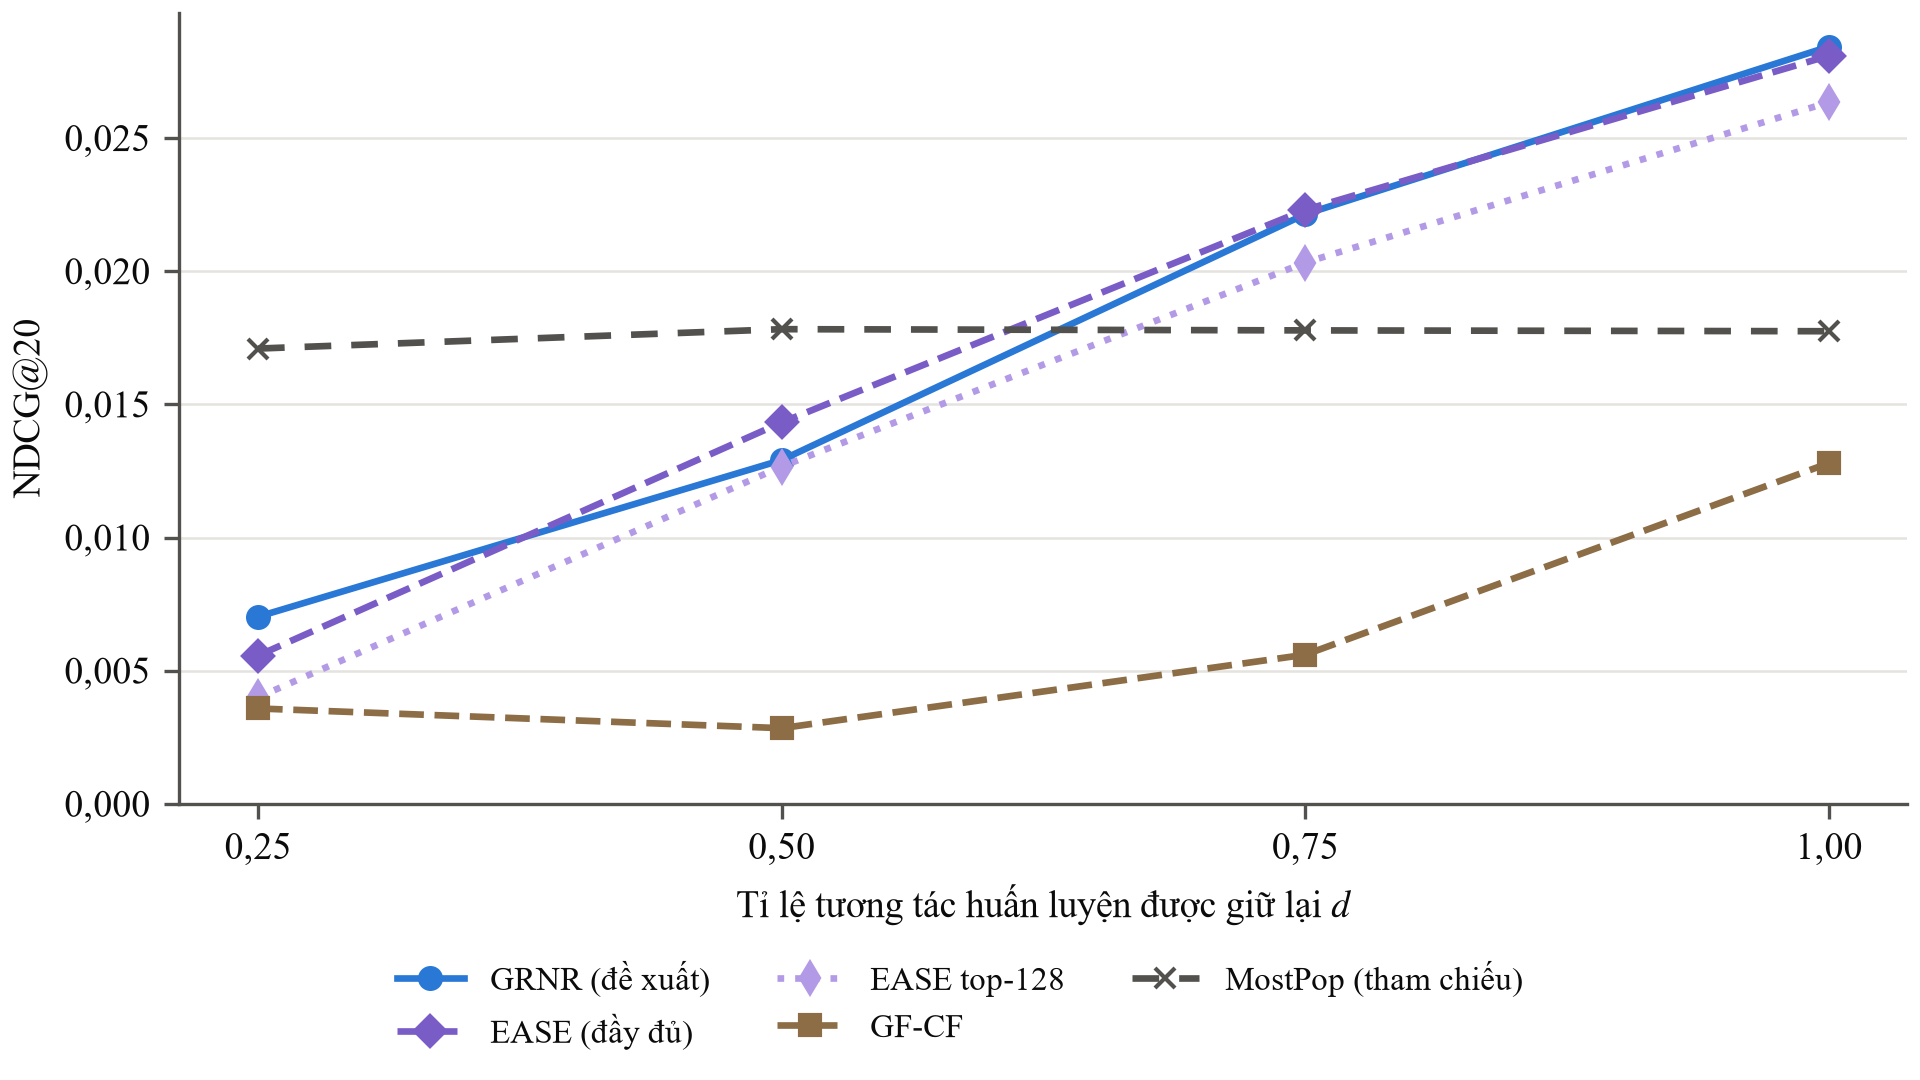
\includegraphics[width=\linewidth,height=0.67\textheight,keepaspectratio]{figures/fig_5_6_GRNR_vs_MostPop.png}
\takeaway{$d=0{,}5$: thấp hơn EASE đầy đủ (9,8\%). $d=0{,}25$: \textbf{cao hơn EASE đầy đủ 26,2\%} (KTC $\Delta$ trên 0), nhưng vẫn \textbf{thấp hơn MostPop 58,9\%}.}
\end{frame}

\begin{frame}{GRNR mất tín hiệu gì khi dữ liệu thưa?}
\centering
{\small\bfseries\color{PrimaryBlue}Chỉ giữ 25\% tương tác không có nghĩa giữ 25\% tín hiệu}\par
\vspace{0.09cm}

\begin{columns}[T,onlytextwidth]

\begin{column}{0.45\textwidth}
    \metric{4,2\%}{Cặp đồng xuất hiện còn lại}
\end{column}
\hfill
\begin{column}{0.45\textwidth}
    \metric{12,7\%}{Sản phẩm không còn láng giềng}
\end{column}

\end{columns}

\vspace{0.10cm}
\begin{tikzpicture}[
 left/.style={draw=PrimaryBlue,rounded corners=4pt,fill=PaleBlue,
 minimum height=1.03cm,text width=4.1cm,align=center,font=\small,inner sep=6pt},
 ar/.style={-Latex,line width=1.3pt,draw=PrimaryBlue}]
\node[left] (l) {\textbf{Có đồng xuất hiện}\\Sản phẩm trong cùng lịch sử};
\node[left,right=1.0cm of l] (r) {\textbf{Khi tín hiệu cạn}\\Ít láng giềng, trọng số khó ước lượng};
\draw[ar] (l) -- (r);
\end{tikzpicture}
\vspace{0.04cm}
\begin{block}{Hệ quả với GRNR (Bảng 5.4)}
\small Số láng giềng trung bình giảm từ \textbf{89,8} xuống \textbf{11,1}. Sản phẩm cô lập chỉ còn hệ số chặn $b_i$ trong điểm số.
\end{block}
\takeaway{Tín hiệu đồng xuất hiện suy giảm mạnh; cần ablation để xác định tác động riêng của $b_i$.}
\end{frame}

\begin{frame}{GRNR: Lợi thế dung lượng gần 190 lần}
\centering
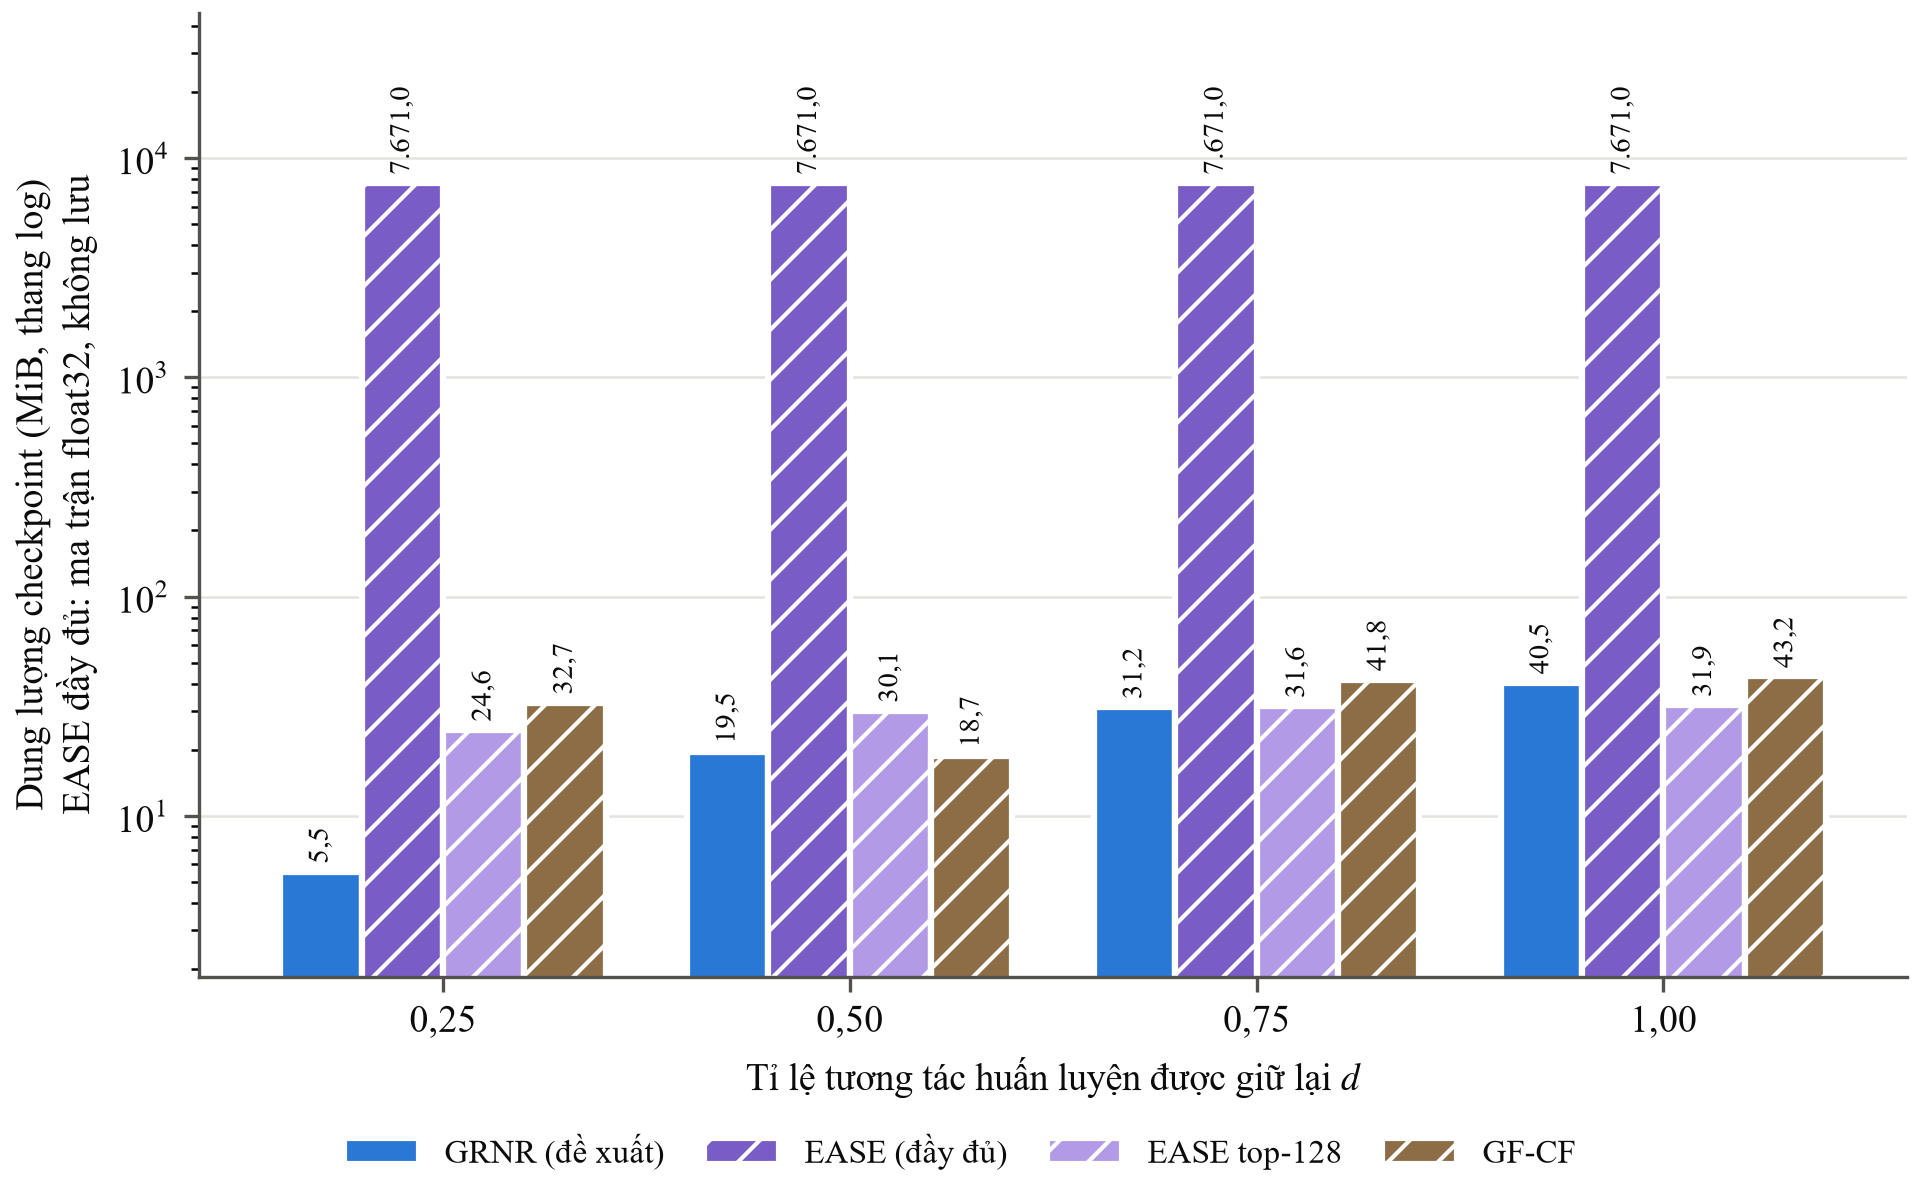
\includegraphics[width=\linewidth,height=0.60\textheight,keepaspectratio]{figures/fig_5_15_GRNR_Memory.png}
\vspace{0.04cm}
\begin{columns}[T,totalwidth=\textwidth]
\column{0.46\textwidth}
\begin{block}{\centering\large\bfseries 40,5 MiB}
\centering\footnotesize Checkpoint GRNR ($d=1$)
\end{block}
\column{0.46\textwidth}
\begin{block}{\centering\large\bfseries 7,5 GiB}
\centering\footnotesize Ma trận EASE đầy đủ (ước tính)
\end{block}
\end{columns}
\shortnote{GRNR nhỏ hơn xấp xỉ 190 lần; thời gian chạy giữa các thiết bị chỉ có ý nghĩa tham khảo.}
\end{frame}

\section{Kết quả DFHF}

\begin{frame}{DFHF tại $d=1$: Dẫn đầu nhóm cần huấn luyện}
\centering
\small
\begin{tabular}{lrr}
\toprule
\textbf{Nhóm cần huấn luyện (test)} & \textbf{NDCG@20} $\uparrow$ & \textbf{Recall@20} $\uparrow$\\
\midrule
\rowcolor{PaleBlue}\textbf{DFHF} & \textbf{0,02724} & \textbf{0,05966}\\
LightGCN & 0,02168 & 0,04870\\
XSimGCL & 0,02561 & 0,05647\\
DirectAU & 0,02407 & 0,05256\\
\bottomrule
\end{tabular}
\vspace{0.37cm}
\begin{block}{Kiểm định NDCG@20}
\small
DFHF $-$ XSimGCL: $+0{,}00163$; KTC 95\% $[+0{,}00111;\,+0{,}00213]$.\\[5pt]
DFHF $-$ DirectAU: $+0{,}00317$; KTC 95\% $[+0{,}00260;\,+0{,}00375]$.
\end{block}
\vspace{0.22cm}
\takeaway{DFHF tốt nhất \textbf{trong nhóm} trên test, hơn cả ba baseline ở mọi mức $d$; chênh lệch còn phụ thuộc ngân sách tuning.}
\end{frame}

\begin{frame}{DFHF theo $d$: Dẫn đầu nhóm, chỉ ngang MostPop khi rất thưa}
\centering
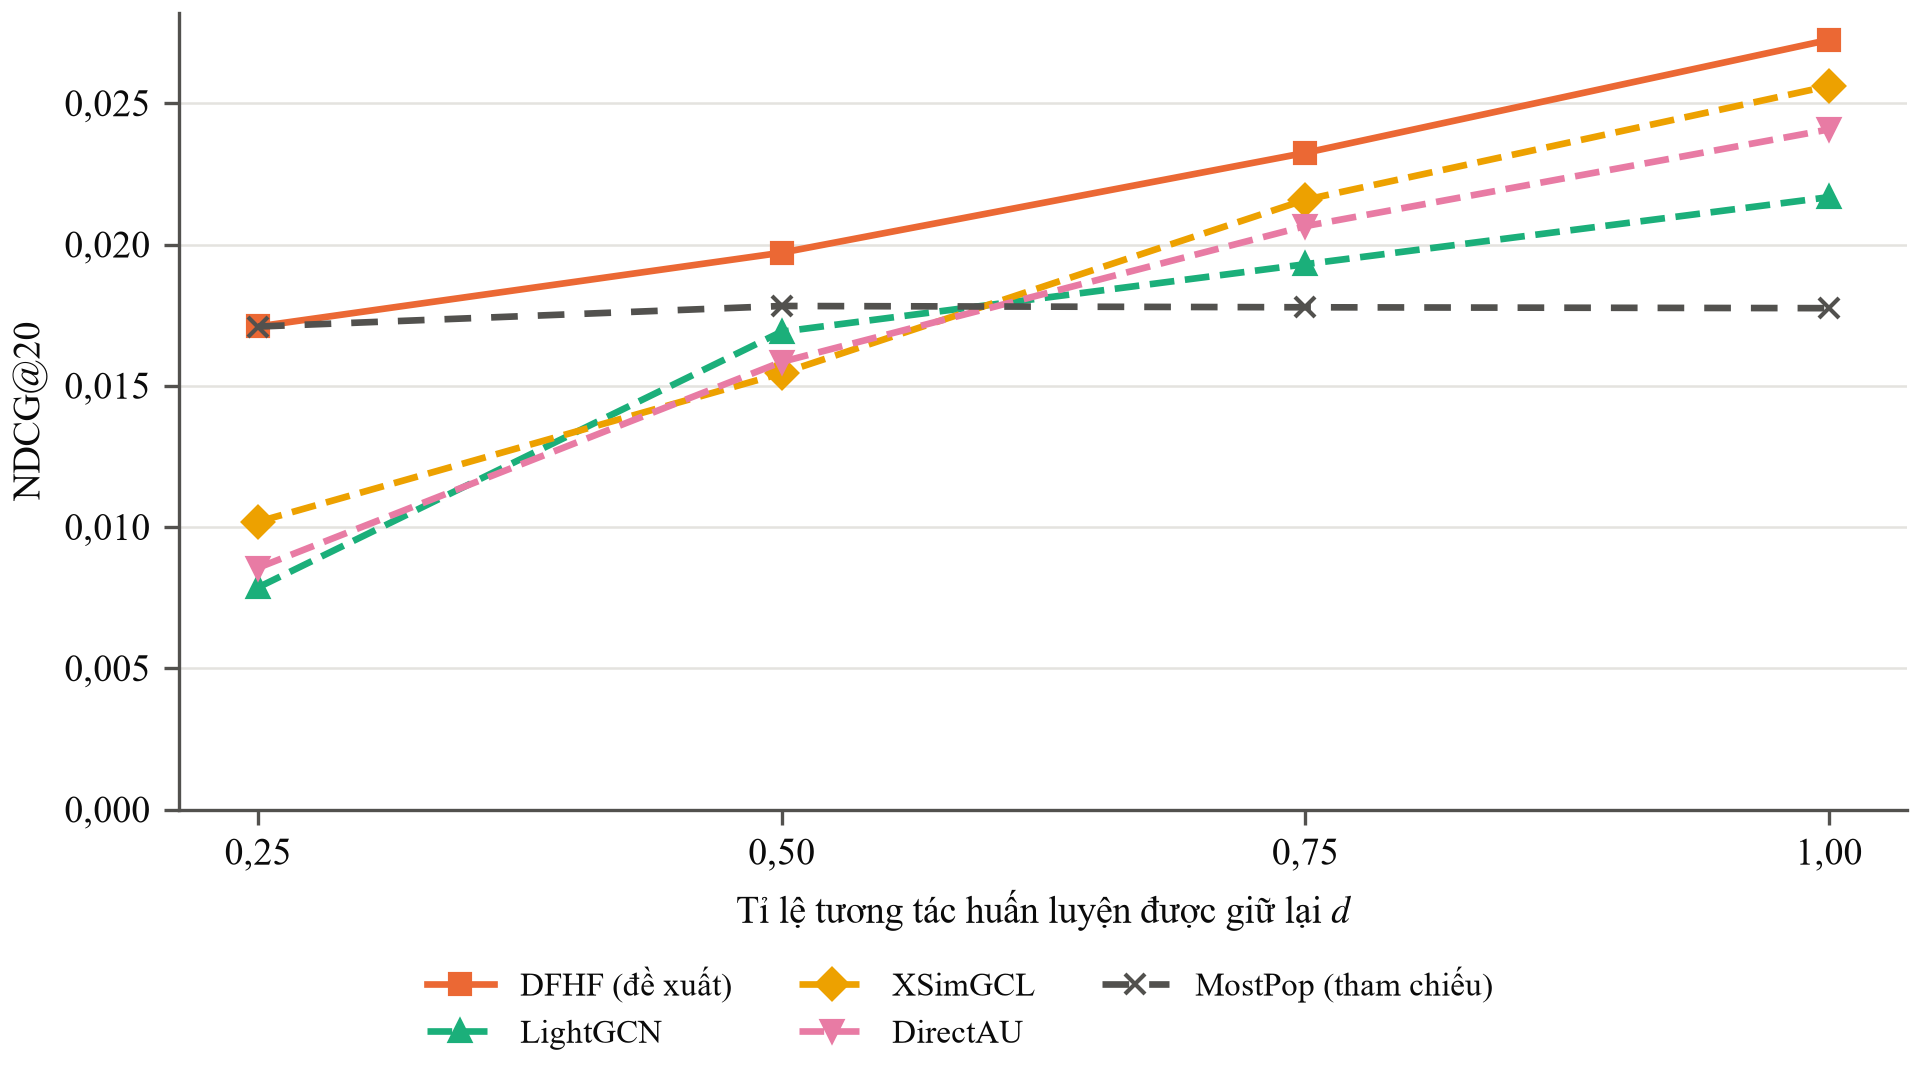
\includegraphics[width=\linewidth,height=0.66\textheight,keepaspectratio]{figures/fig_5_21_DFHF_vs_MostPop.png}
\takeaway{Ở $d=0{,}25$, DFHF hơn cả ba baseline cùng nhóm nhưng \textbf{chỉ bằng MostPop} (0,01710); MostPop là mốc tham chiếu.}
\end{frame}

\begin{frame}{DFHF ($d=0{,}25$): 68\% người dùng chỉ còn 1 tương tác}
\centering
\begin{columns}[T,totalwidth=\textwidth]
\column{0.43\textwidth}
{\color{PrimaryBlue}\fontsize{27}{32}\selectfont\bfseries 68\%}\par
\small Người dùng warm bậc 1\par
\footnotesize ($n=72.889$, $d=0{,}25$, test)
\column{0.55\textwidth}
\begin{block}{Cơ chế DFHF}
\vspace{-0.16cm}\[q_u=0\Rightarrow s(u,i)=b_i\]\vspace{-0.06cm}
\footnotesize Không dùng tín hiệu từ lịch sử đơn.
\end{block}
\end{columns}
\vspace{0.08cm}
\begin{block}{NDCG@20 theo lịch sử bậc 1}
\vspace{-0.1cm}
\centering
\small
\renewcommand{\arraystretch}{0.86}
\begin{tabular}{lr}
\toprule
\textbf{Phương pháp} & \textbf{NDCG@20}\\
\midrule
\rowcolor{PaleBlue} DFHF (chỉ hệ số chặn) & \textbf{0,01757}\\
MostPop (không cá nhân hóa) & \textbf{0,01746}\\
LightGCN & 0,00788\\
XSimGCL & 0,01041\\
DirectAU & 0,00849\\
\bottomrule
\end{tabular}
\end{block}
\vspace{0.04cm}
\takeaway{DFHF bậc 1 gần MostPop; lợi thế so với baseline \textbf{không chứng minh} cá nhân hóa tốt hơn.}
\end{frame}

\begin{frame}{DFHF: Kết quả phụ thuộc checkpoint}
\centering
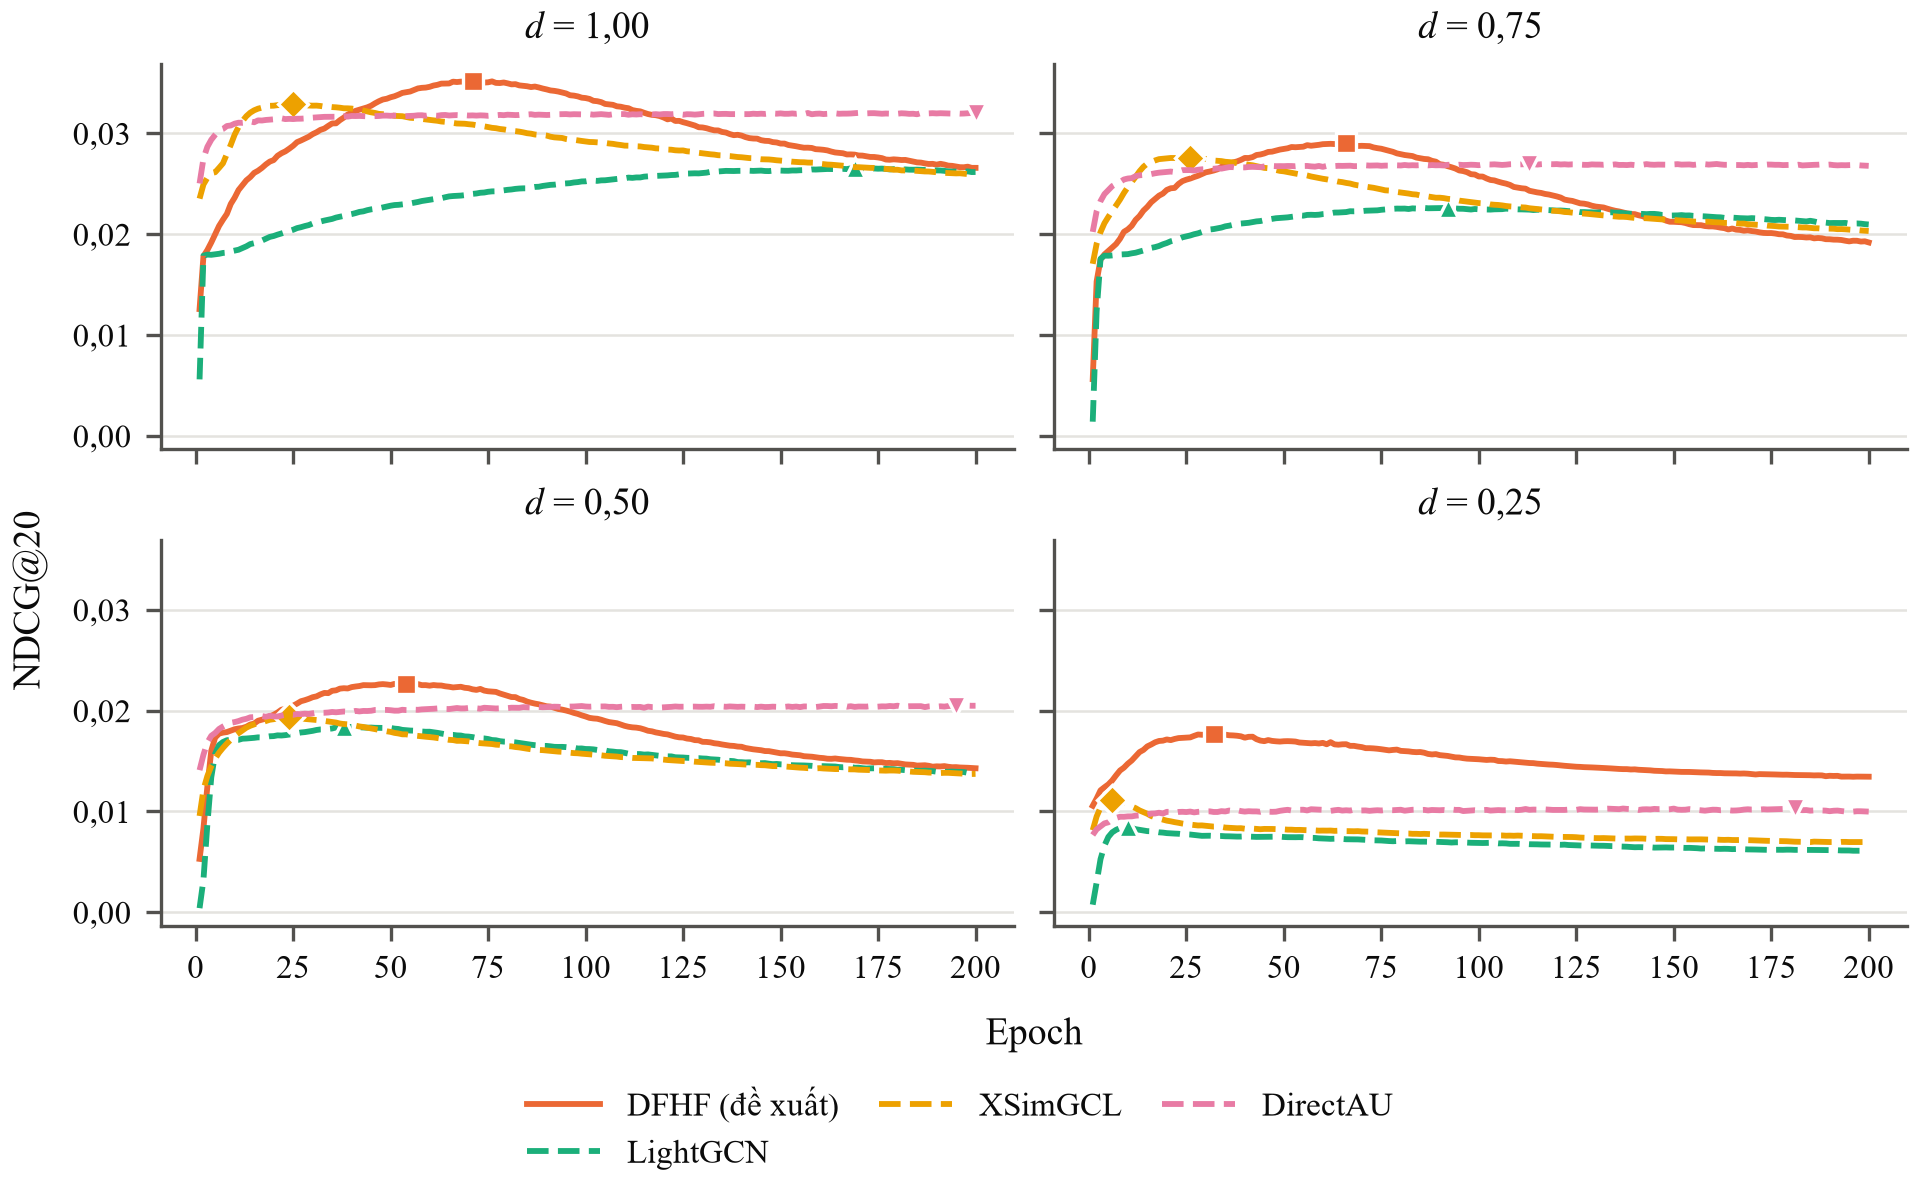
\includegraphics[width=\linewidth,height=0.55\textheight,keepaspectratio]{figures/fig_5_30_DFHF_LearningCurve.png}
\begin{columns}[T,totalwidth=\textwidth]
\column{0.48\textwidth}
\begin{block}{\centering\bfseries Chọn epoch 71}
\centering\large 0,03519\par\footnotesize NDCG@20 validation
\end{block}
\column{0.48\textwidth}
\begin{block}{\centering\bfseries Epoch cuối}
\centering\large 0,02658\par\footnotesize NDCG@20 validation
\end{block}
\end{columns}
\shortnote{Giảm 24,5\% sau đỉnh; trên test, epoch 71 đạt 0,02724, cao nhất nhóm.}
\end{frame}

\section{Thảo luận và kết luận}

\begin{frame}{Hai chế độ dữ liệu - Bài học chung}
\centering
\vspace{0.15cm}
\begin{tikzpicture}[
 stage/.style={draw=PrimaryBlue,rounded corners=5pt,fill=PaleBlue,
 minimum height=1.78cm,text width=3.0cm,align=center,font=\small,inner sep=7pt},
 arr/.style={-Latex,draw=PrimaryBlue,line width=1.4pt}]
\node[stage] (a) {\bfseries Dữ liệu đủ dày\\[2pt]$d=1$\\[4pt]Tốt nhất mỗi nhóm vượt MostPop \textbf{54--60\%}};
\node[stage,right=0.44cm of a] (b) {\bfseries Dữ liệu giảm\\[2pt]$d=0{,}5$\\[4pt]Chỉ \textbf{DFHF} còn vượt MostPop (11\%)};
\node[stage,right=0.44cm of b] (c) {\bfseries Rất thưa\\[2pt]$d=0{,}25$\\[4pt]\textbf{Không mô hình nào} hơn MostPop};
\draw[arr] (a) -- (b);\draw[arr] (b) -- (c);
\end{tikzpicture}
\vspace{0.39cm}

\begin{columns}[T,onlytextwidth]

    \begin{column}{0.47\textwidth}
        \begin{block}{GRNR: Thiếu kết nối}
            \small
            Chỉ còn \textbf{4,2\%} cặp đồng xuất hiện. Ít láng giềng để học hệ số.
        \end{block}
    \end{column}

    \hfill

    \begin{column}{0.47\textwidth}
        \begin{block}{DFHF: Lùi về chặn}
            \small \textbf{68\%} người dùng chỉ còn 1 tương tác: xếp hạng bằng $b_i$.
        \end{block}
    \end{column}

\end{columns}
\vspace{0.18cm}
\takeaway{Trên dữ liệu này, \textbf{độ dày dữ liệu} quyết định lợi ích cá nhân hóa nhiều hơn việc chọn một mô hình phức tạp.}
\end{frame}

\begin{frame}{Demo: Gợi ý cho người dùng có sẵn}
\centering

\vspace{-0.06cm}

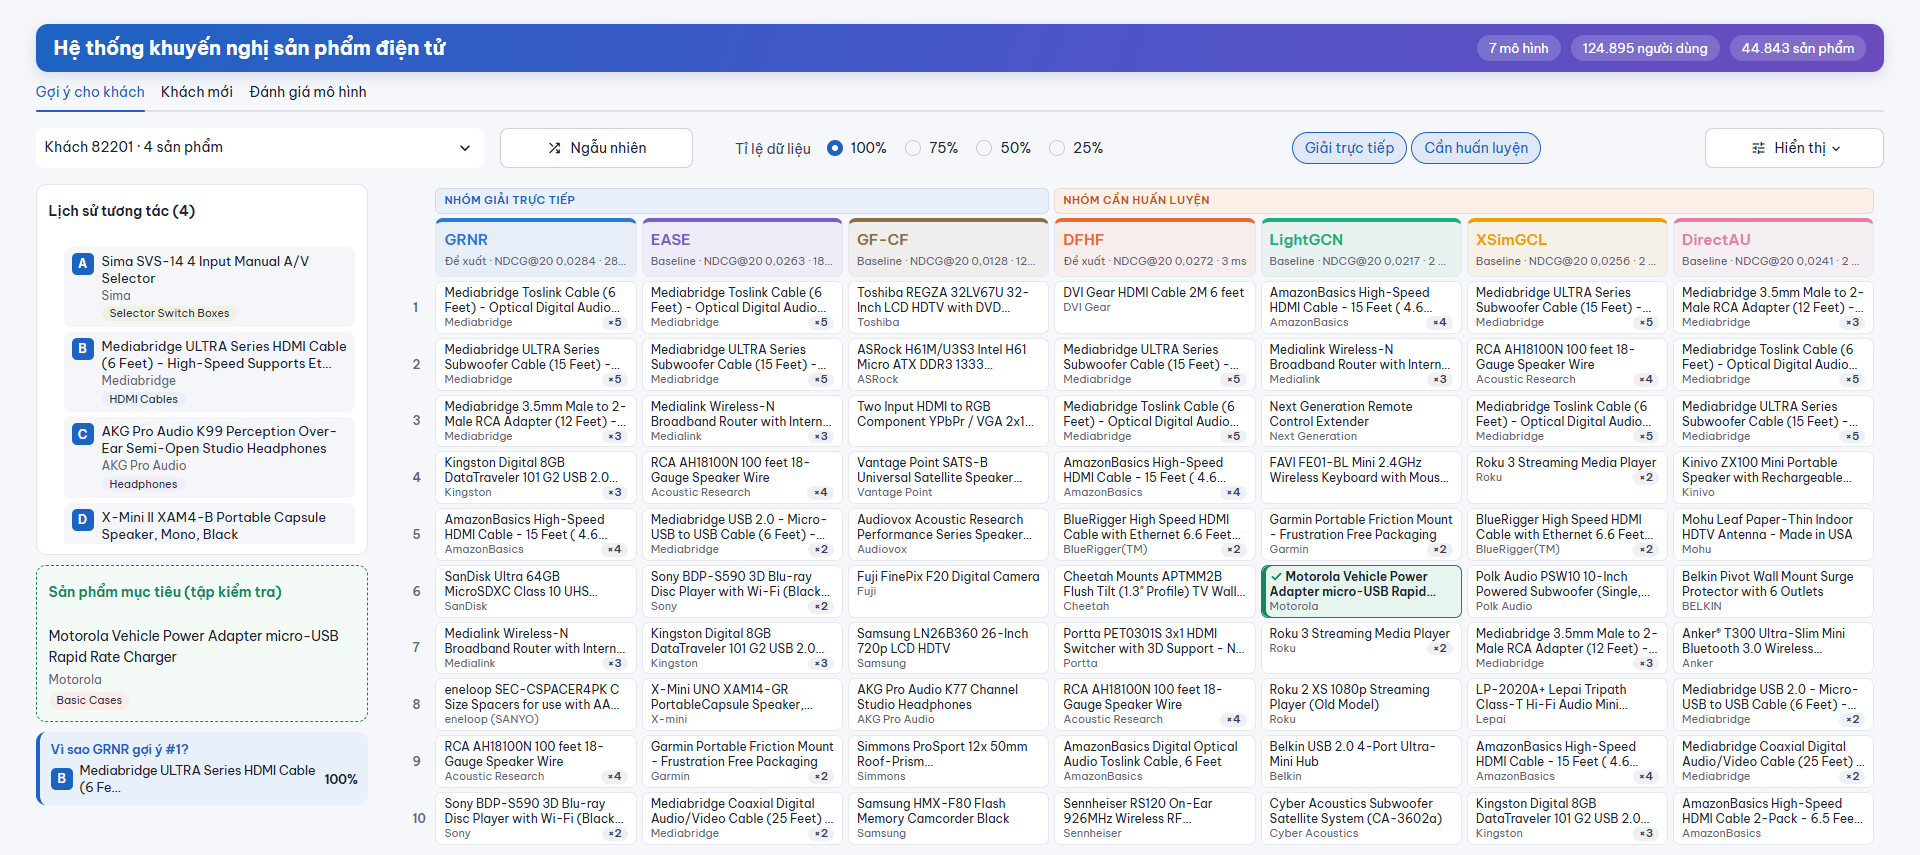
\includegraphics[
    width=\linewidth,
    height=0.66\textheight,
    keepaspectratio
]{figures/anh_1.png}

\vspace{0.05cm}

\takeaway{
Từ lịch sử của người dùng, hệ thống hiển thị
\textbf{Top-10 của 7 mô hình} và sản phẩm mục tiêu.
Với GRNR, ô ``Vì sao gợi ý \#1?''
thể hiện đóng góp từ các sản phẩm trong lịch sử.
}

\end{frame}

\begin{frame}{Demo: Gợi ý cho khách mới}
\centering

\vspace{-0.06cm}

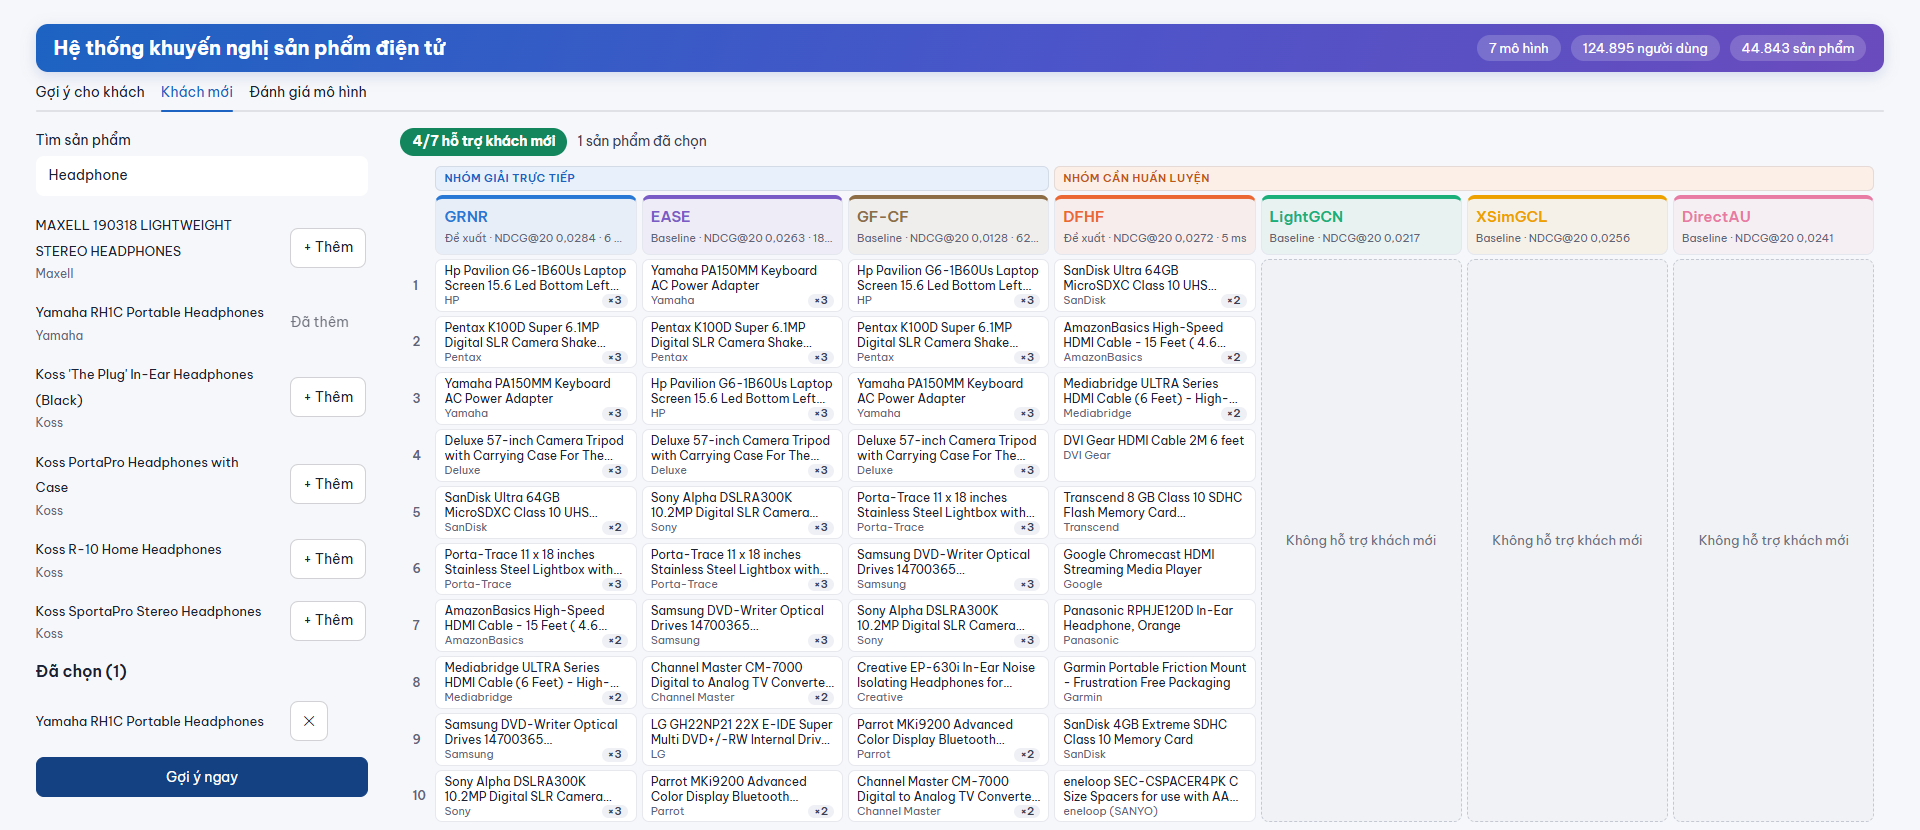
\includegraphics[
    width=\linewidth,
    height=0.66\textheight,
    keepaspectratio
]{figures/anh_2.png}

\vspace{0.05cm}

\takeaway{
Khách mới có thể \textbf{tìm và thêm sản phẩm}
để tạo lịch sử.
\textbf{4/7 mô hình} chấm điểm lịch sử mới
mà không huấn luyện lại;
trong ví dụ một tương tác,
DFHF xếp hạng theo hệ số chặn $b_i$.
}

\end{frame}

\begin{frame}{Demo: Gợi ý và lý do gợi ý của GRNR}
\centering
\begin{columns}[T,totalwidth=\textwidth]
\column{0.50\textwidth}
\centering
{\footnotesize\bfseries\color{PrimaryBlue}Sản phẩm mục tiêu và lý do GRNR gợi ý}\par\vspace{0.13cm}
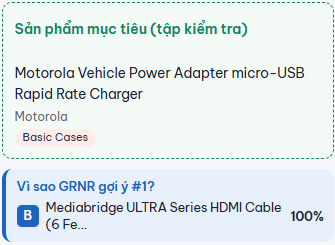
\includegraphics[width=0.96\linewidth,height=0.53\textheight,keepaspectratio]{figures/demo_focus_reason.png}

\column{0.48\textwidth}
\centering
{\footnotesize\bfseries\color{PrimaryBlue}Top-3 gợi ý của GRNR}\par\vspace{0.13cm}
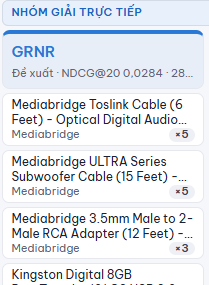
\includegraphics[width=0.98\linewidth,height=0.53\textheight,keepaspectratio]{figures/demo_focus_grnr_top3.png}
\end{columns}
\vspace{0.09cm}
\takeaway{Từ lịch sử 4 tương tác, demo dùng checkpoint sẵn có để xếp hạng. Ô ``Vì sao GRNR gợi ý \#1?'' cho thấy đóng góp từ lịch sử, \textbf{không} là diễn giải nhân quả.}
\end{frame}

\begin{frame}{Kết luận gắn với bốn câu hỏi nghiên cứu}
\small
\begin{enumerate}\setlength\itemsep{0.29cm}
\item \textbf{Chất lượng:} GRNR hơn EASE top-128; chưa chứng minh hơn EASE đầy đủ. DFHF dẫn đầu nhóm cần huấn luyện trên test.
\item \textbf{Dữ liệu thưa:} ở $d=0{,}25$, \textbf{không mô hình nào hơn MostPop}; lợi thế DFHF chủ yếu từ hệ số chặn.
\item \textbf{Chi phí:} GRNR nhỏ hơn EASE đầy đủ \textbf{khoảng 190 lần}; DFHF huấn luyện chậm nhất nhóm, nhạy checkpoint.
\item \textbf{Lịch sử mới:} cả hai phương pháp tính được điểm không cần huấn luyện lại; demo minh họa phân rã điểm GRNR.
\end{enumerate}
\vspace{0.12cm}
\takeaway{Kết quả đo trên \textbf{test độc lập}, nhưng chỉ với một bộ dữ liệu và một seed, nên vẫn là \textbf{kết quả khám phá}.}
\end{frame}

\begin{frame}{Hạn chế quan trọng và ưu tiên tiếp theo}
\small

\begin{columns}[T,onlytextwidth]

    \begin{column}{0.49\textwidth}
        \begin{block}{Cần thận trọng}
            \begin{itemize}\setlength\itemsep{6pt}
            \item \textbf{Một bộ dữ liệu, một seed}
            \item Ngân sách \textbf{tinh chỉnh baseline không cân bằng}
            \item \textbf{DirectAU có dấu hiệu chưa hội tụ}
            \item \textbf{GF-CF thấp bất thường}: cần kiểm tra cài đặt/cấu hình
            \end{itemize}
        \end{block}
    \end{column}

    \hfill

    \begin{column}{0.47\textwidth}
        \begin{block}{Ưu tiên phát triển}
            \begin{enumerate}\setlength\itemsep{6pt}
            \item Nhiều seed, thêm bộ dữ liệu.
            \item Kiểm lại GF-CF; tuning cùng ngân sách, huấn luyện DirectAU đủ lâu.
            \item Ablation từng thành phần GRNR/DFHF.
            \item Kết hợp \textbf{MostPop dự phòng} khi lịch sử quá ngắn.
            
            \end{enumerate}
        \end{block}
    \end{column}

\end{columns}


\vspace{0.18cm}
\vspace{0.18cm}
\begin{center}
\begin{minipage}{0.91\textwidth}
\centering\footnotesize\bfseries\color{PrimaryBlue}
Cần kiểm chứng: phương án dự phòng và khả năng khái quát sang dữ liệu khác.
\end{minipage}
\end{center}
\end{frame}

\begin{frame}[plain]
\vfill
\begin{center}
{\LARGE\bfseries\color{PrimaryBlue}XIN CẢM ƠN THẦY CÔ VÀ CÁC BẠN!}\\[0.65cm]
{\large Nhóm sẵn sàng trao đổi và trả lời câu hỏi.}\\[0.32cm]
{\normalsize Hệ thống khuyến nghị sản phẩm điện tử\\
bằng hồi quy lân cận và khuếch tán trên đồ thị}
\end{center}
\vfill
\end{frame}

\end{document}
